\documentclass{article}
\usepackage{hyperref}
\usepackage[margin=1in]{geometry}
\usepackage{graphicx}
\begin{document}
\author{Tan Ren Jie}
\title{Convexity Analysis of Weight Potential of the XOR Problem}
\maketitle
\section{Introduction}
The XOR problem is the classic example of a linearly inseparable problem. It is also commonly used to show the limitation of a single-layer perceptron. In this paper, we would try to understand more deeply about the mathematics of the XOR problem.
\section{Bias matters}
Initially, we undermined the importance of the bias terms. We realized that by excluding the bias terms, the MLP is unable to achieve a better cost than $0.25$ even for a network with $10$ hidden nodes optimized by Adam. \\ \\
In effect, the bias terms plays the role of shifting the activation function to the left or right, which is very often of the time critical for successful learning. This can be seen by looking more closely at the equations:
$$h1 = \sigma(W1^TX + b1)$$
$$pred = \sigma(W2^Th1 + b2)$$
$$MSE = (Y - pred)^2.mean()$$

\begin{figure}[h]
	\begin{center}
		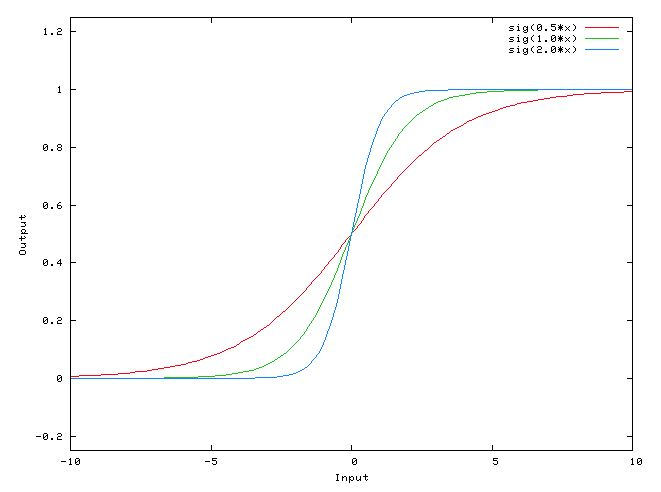
\includegraphics[scale = 0.5]{activation_wo_bias.jpg}
		\caption{Sigmoid activation without bias terms}
	\end{center}
\end{figure}
Changing the weights essentially changes the "steepness" of the sigmoid. That's useful, but what if you wanted the network to output 0 when x is 2? Just changing the steepness of the sigmoid won't really work -- you want to be able to shift the entire curve to the right. \\ \\
This is somehow similar to the $b$ term of a linear function
$$y = ax + b$$
It allows you to move the line up and down to fit the prediction with the data better. Without $b$ the line always goes through the origin $(0, 0)$ and you may get a poorer fit. \\ \\
\begin{figure}[h]
	\begin{center}
		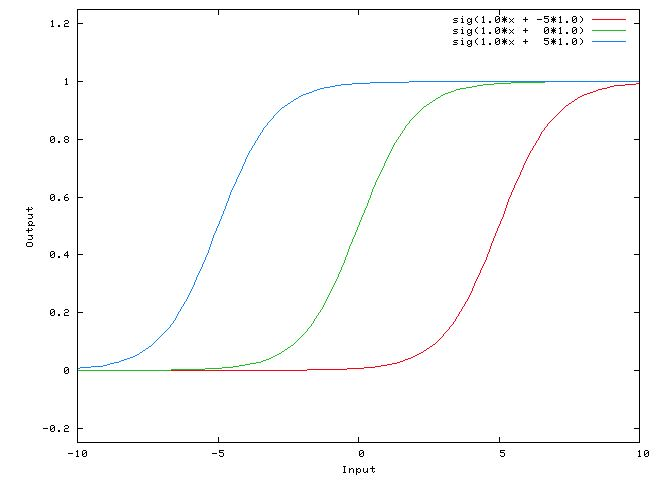
\includegraphics[scale = 0.5]{activation_w_bias.jpg}
		\caption{Sigmoid activation with bias terms}
	\end{center}
\end{figure}
Image credit: Nate Kohl, user of Stackoverflow from the following post
https://stackoverflow.com/questions/2480650/role-of-bias-in-neural-networks
\section{Vanilla Gradient Descent Does'nt Work}
It is observed that the Vanilla Gradient Descent is not able to achieve a better cost than $0.25$ even for the MLP with 10 hidden nodes. This could be due to the symmetry of the weight potential where weights get stuck in a ring of saddle points or valleys. \\ \\
By adding the respective bias terms and using Adam, we were able to achieve a cost lower than $0.25$ where we suspect is the global minimum. 
\section{Results}
Implementing the Adam optimiser and introducing the bias terms, the following plots were obtained. 
\begin{figure} [H]
	\begin{center}
	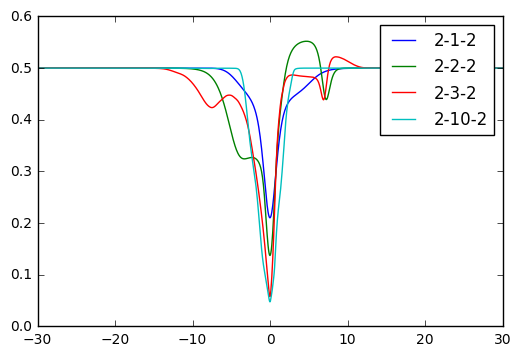
\includegraphics[scale =1]{Convexity_analysis_weight_potential.png}
	\caption{Weight Potential for a 3-layer MLP with hidden nodes = 1,2,3 and 10}
	\end{center}
\end{figure}
The following plots where generated by first optimizing the weights and varying the optimized weights between $-30 \rightarrow 30$ with the optimized weights centered at $x = 0$ in the plot. The $y$-axis is the MSE of the XOR problem
\end{document}